\documentclass[border=10pt]{standalone}

\usepackage{tikz}
\usepackage{tikzsymbols}
\usetikzlibrary{calc,patterns,shapes.geometric}

\def\centerarc[#1](#2)(#3:#4:#5){\draw[#1] ($(#2)+({#5*cos(#3)},{#5*sin(#3)})$) arc (#3:#4:#5);}

\begin{document}
	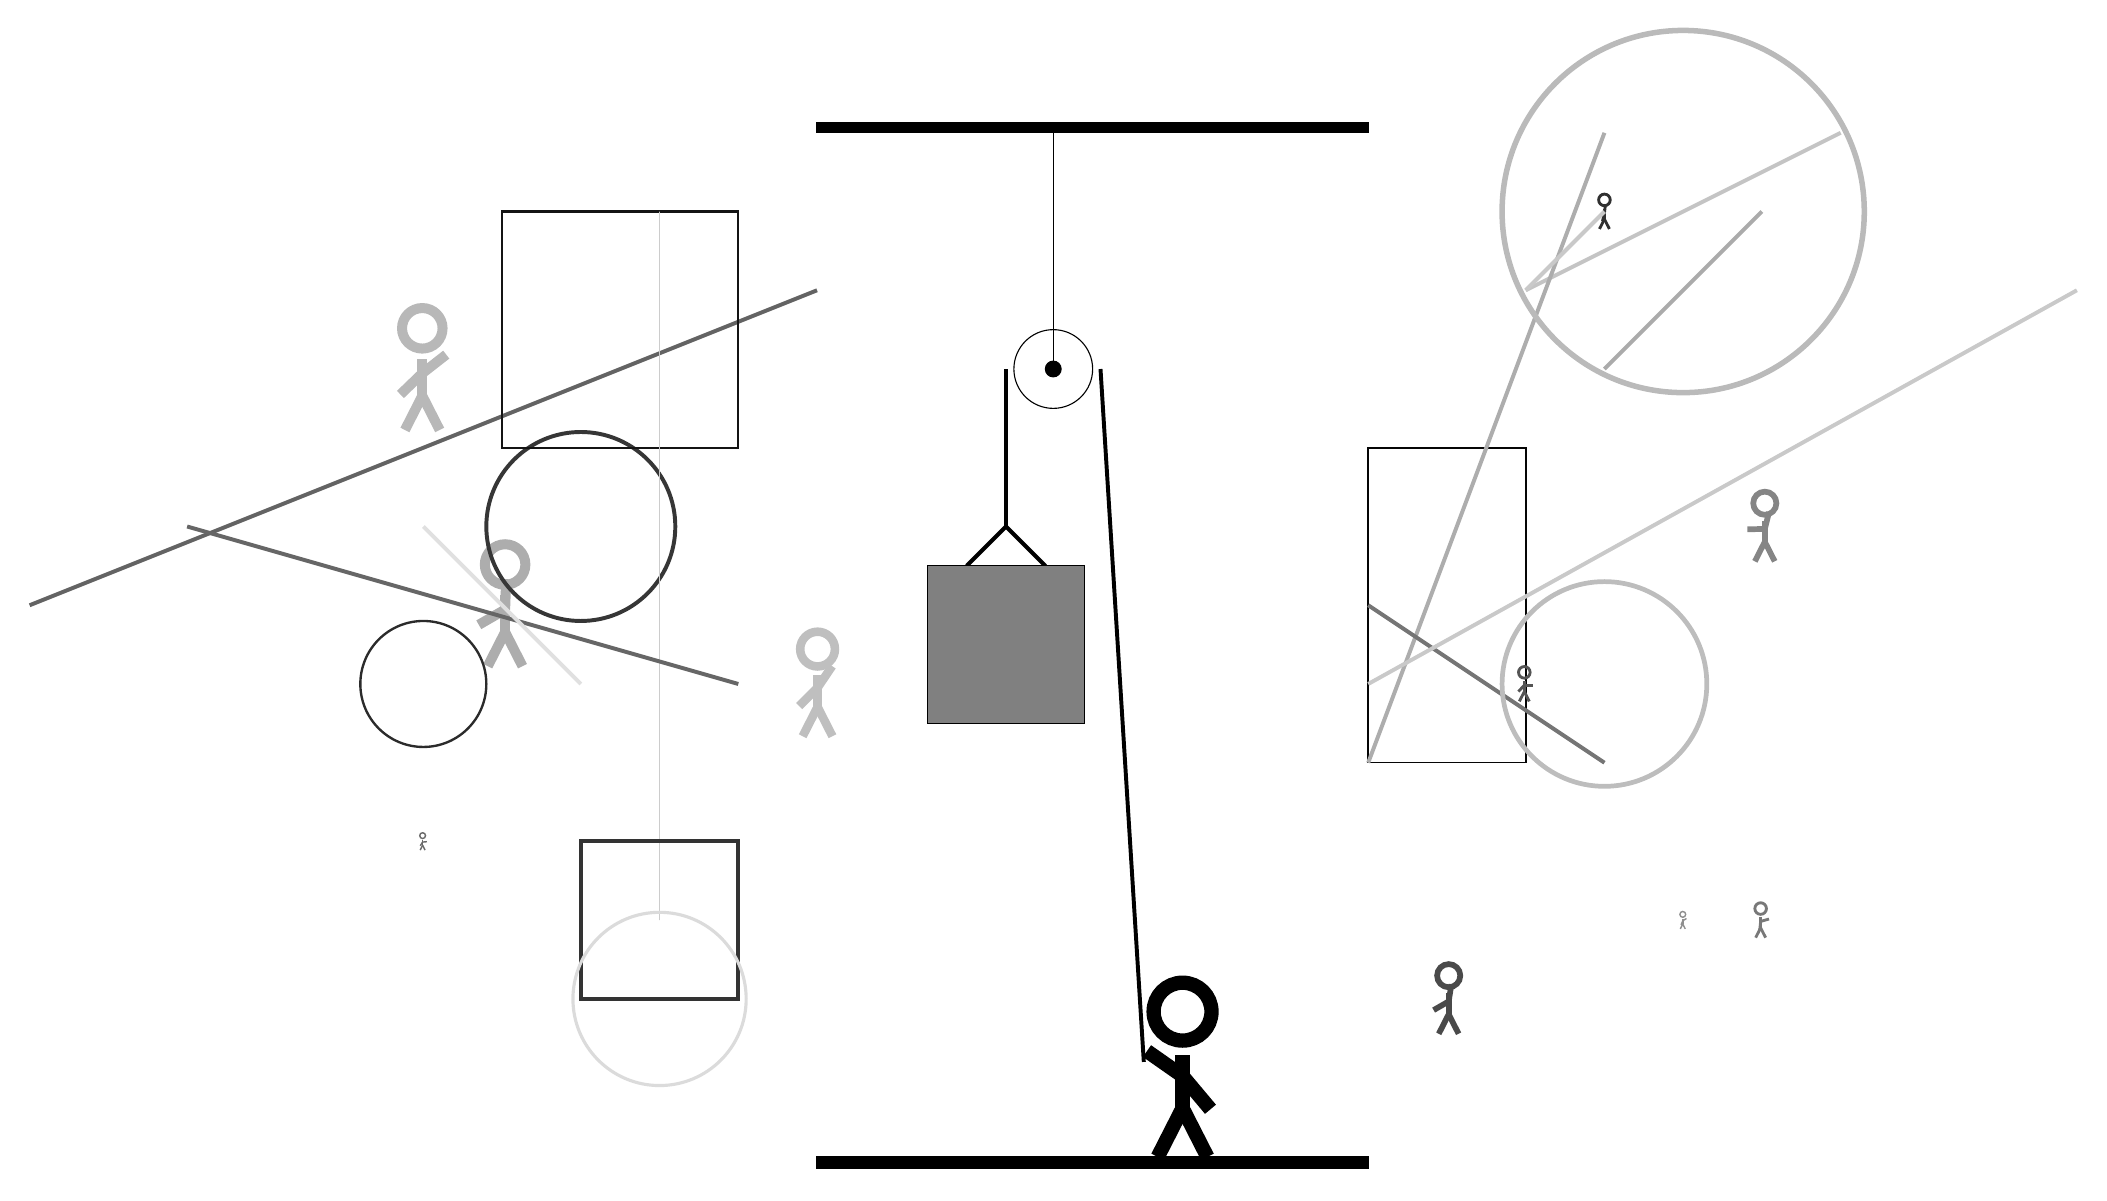
\begin{tikzpicture}
		%%%%% START %%%%%
		
		\draw[fill=black] (-2, 10) rectangle (5, 10.125);
		
		\draw (1, 7) circle (0.5);
		\draw[fill=black] (1, 7) circle (0.1);
		\draw (1, 10) -- (1, 7);
		
		\draw [line width=0.6mm, color=black!79](-4, 7) circle (0.0);
		
		\draw[line width=0.5mm, color=black!10](-5, -1) -- (-5, 1);
		\node[line width=0.2mm, color=black!48] at (10, 5) {\Strichmaxerl[4][1][76]};
		\node[line width=0.5mm, color=black!81] at (8, 9) {\Strichmaxerl[2][77][83]};
		\node[line width=0.5mm, color=black!32] at (-6, 4) {\Strichmaxerl[7][30][88]};
		\draw[line width=0.2mm, color=black!98] (7, 2) rectangle (5, 6);
		\draw[line width=0.5mm, color=black!61](-2, 8) -- (-12, 4);
		\draw [line width=0.5mm, color=black!79](-5, 5) circle (1.2);
		\draw[line width=0.5mm, color=black!23](7, 8) -- (11, 10);
		\node[line width=0.2mm, color=black!67] at (7, 3) {\Strichmaxerl[2][47][0]};
		\draw [line width=0.3mm, color=black!83](-7, 3) circle (0.8);
		\node[line width=0.2mm, color=black!44] at (9, 0) {\Strichmaxerl[1][67][32]};
		\draw[line width=0.5mm, color=black!32](8, 10) -- (5, 2);
		\draw[line width=0.5mm, color=black!54](5, 4) -- (8, 2);
		\node[line width=0.2mm, color=black!25] at (-2, 3) {\Strichmaxerl[6][45][56]};
		\draw[line width=0.5mm, color=black!33](8, 7) -- (10, 9);
		\draw [line width=0.6mm, color=black!26](8, 3) circle (1.3);
		
		\draw[line width=0.3mm, color=black!92] (-3, 6) rectangle (-6, 9);
		\draw[line width=0.2mm, color=black!20] (-4, 0) rectangle (-4, 9);
		\draw[line width=0.5mm, color=black!21](5, 3) -- (14, 8);
		\node[line width=0.4mm, color=black!53] at (10, 0) {\Strichmaxerl[2][84][16]};
		
		\draw[line width=0.5mm, color=black!60](-3, 3) -- (-10, 5);
		\draw[line width=0.5mm, color=black!80] (-3, 1) rectangle (-5, -1);
		\draw [line width=0.7mm, color=black!27](9, 9) circle (2.3);
		\draw [line width=0.4mm, color=black!14](-4, -1) circle (1.1);
		
		\draw[line width=0.5mm, color=black!12](-7, 5) -- (-5, 3);
		\node[line width=0.4mm, color=black!28] at (-7, 7) {\Strichmaxerl[7][44][38]};
		\node[line width=0.5mm, color=black!58] at (-7, 1) {\Strichmaxerl[1][57][5]};
		\draw [line width=0.7mm, color=black!68](-7, 5) circle (0.0);
		
		\node[line width=0.4mm, color=black!71] at (6, -1) {\Strichmaxerl[4][30][81]};
		\draw[line width=0.5mm, color=black!21](8, 9) -- (7, 8);
		
		
		\draw[line width=0.5mm] (-0.1, 4.5) -- (0.4, 5.0) -- (0.9, 4.5);
		\draw[fill=black!50] (-0.6, 4.5) rectangle (1.4, 2.5);
		
		\draw[line width=0.5mm] (0.4, 7) -- (0.4, 5.0);
		\centerarc[line width=0.5mm](1, 7)(0:180:0.6);
		\draw[line width=0.5mm](1.6, 7) -- (2.15, -1.8);
		
		\node at (2.6, -1.9) {\Strichmaxerl[10][-35][-50]};
		
		\draw[fill=black] (-2, -3) rectangle (5, -3.15);
		
		%%%%% END %%%%%
	\end{tikzpicture}
\end{document}